\section{Marco Teorico}

\noindent En esta sección se busca explicar conceptos importantes que son utilizados durante el documento.

\subsection{Dirección MAC}

\noindent Cuando se habla de una dirección MAC se hace referencia de la dirección física de un dispositivo la cual es un identificador único que cada fabricante le asigna a la tarjeta de red de sus equipos. La dirección MAC está formadas por 48 bits representados generalmente por dígitos hexadecimales y tienen la forma: \verb|00:1e:c2:9e:28:6b|. Las direcciones MAC pueden ser utilizadas para permitir o denegar el acceso de determinados dispositivos a una red \cite{MAC}.


\subsection{Herramientas de Linux}

\noindent A continuación se describen las herramientas/programas utilizadas en el documento, estas herramientas o programadas de análisis son en su mayoría propias del sistema operativo Linux:

\begin{enumerate}
    \item \textbf{nmap} - Se utilizará para averiguar la topología de la red.
    \item \textbf{ifconfig} - Es la utilidad principal usada para configurar las interfaces de red.
    \item \textbf{Iperf3} - Es una utilidad para medir la velocidad de un enlace en internet.
    \item \textbf{Wireshark} - Es un analizador de protocolos que permite realizar capturas de tráfico de la red en tiempo real y obtener todos los datos de cada paquete involucrado.
\end{enumerate}


\subsection{Protocolo ARP}

\noindent El Address Resolution Protocol (protocolo de resolución de direcciones) es un protocolo de importancia en la transmisión de tramas por el internet debido a que ayuda a obtener las direcciones físicas de los dispositivos (lo que no puede hacer el protocolo de internet) además de almacenar en caché estas direcciones. Este protocolo envía una consulta a la dirección de difusión de la red y se espera que cada dispositivo responda a esa consulta. En síntesis, este protocolo permite que la dirección de internet sea independiente de la dirección de los dispositivos conectaos por LAN, disponibilizado la dirección física. 

\subsubsection{Tablas ARP}

\noindent ARP se encarga de la traducción de las direcciones IP a direcciones MAC por medio de tablas ARP. Sería una especie de base de datos donde se guarda la información de la ip y la MAC de un dispositivo. Para ser técnicos esta información es guardada en la caché y al estar en la caché se borran cada cierto tiempo. 

\begin{figure}[!h]
	\centering
	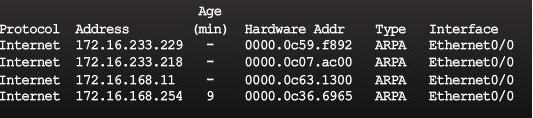
\includegraphics[scale=0.9]{images/arpexample.png}
	\caption{Imagen de ejemplo de una talba ARP}
	\label{arpexa}
\end{figure}

\noindent En general estas tablas poseen la información de la ip del dispositivo y la dirección física o MAC

